\chapter{Punktesortierung in Schachbrettmustern}
\label{sec:schachbrettAlg} 

\section{Algorithmus zur Punktesortierung in verzeichneten Schachbrettbildern}

In diesem Teil der Masterthesis soll am Ende ein Algorithmus entstehen, welcher durch einen bereits bestehenden Algorithmus zur Detektion von Eckpunkten eines Schachbretts, eine Liste an Eckpunkten bekommt und diese auf deren Nachbarschaftsverhältnisse prüft. Die Schachbretter können dabei sowohl Kissen- als auch Tonnennverzeichnungen aufweisen und oder perspektivisch verzerrt sein. Mit den Algorithmus sollen Punkte wissen in welchen Reihen sie sich sowohl in x- als auch y-Richtung befinden. Jeder Punkt bekommt also eine Indexnummer in x-, sowie y-Richtung beziehungsweise in unserem Beispiel wird die y-Koordinate als \textit{j} bezeichnet und die x-Koordinate als \textit{i}, zugewiesen. Jeder Punkt bekommt mit Hilfe von den Mathematica eigenen \textit{Associations} einen \textit{Key} mit \textit{NeighbourJ} und \textit{NeighbourI} zugeteilt. Mit Hilfe dieser \textit{Keys} kann dann später bei einem Stereobildpaar zum Beispiel die Korrespondierenden Eckpunkte der Schachbretter rausgesucht werden, was vielleicht genauere Ergebnisse liefert also die Suche von Hand. Des weiteren kann dieser Algorithmus in späteren Projekten vielleicht bei der Rausrechnung von Verzeichnungen hilfreich sein.\\

\subsection{Vorläufiges Klassendiagramm}

\begin{minipage}{\linewidth}
	\centering
	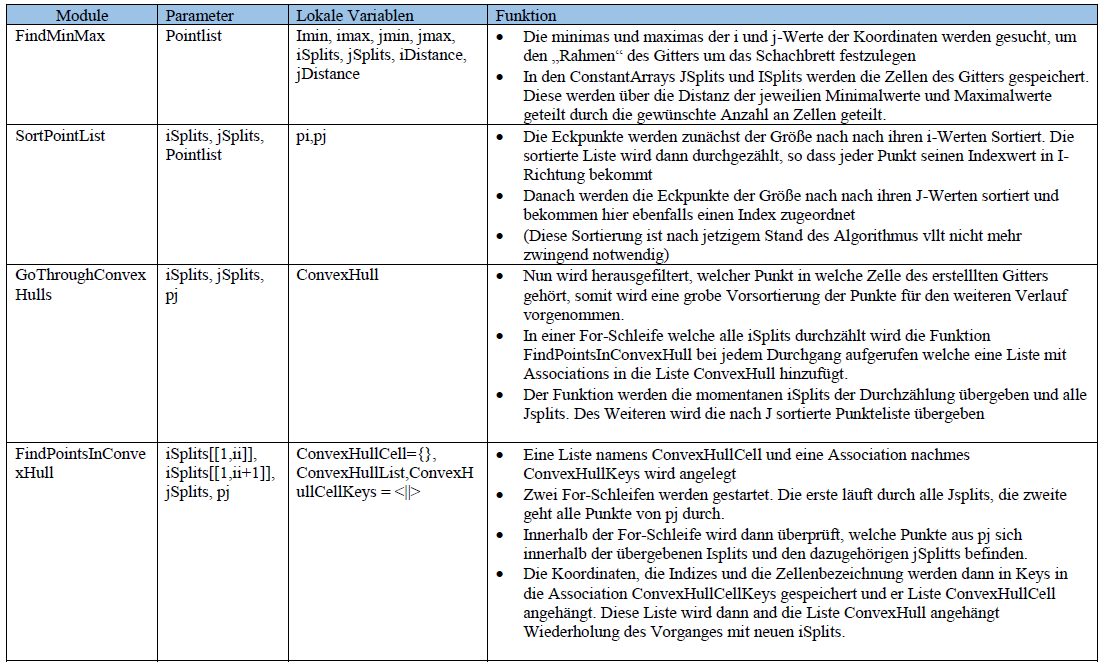
\includegraphics[width=1\linewidth]{images/KD1.png}
	\captionof{figure}{Klassendiagramm}
\end{minipage}
\begin{minipage}{\linewidth}
	\centering
	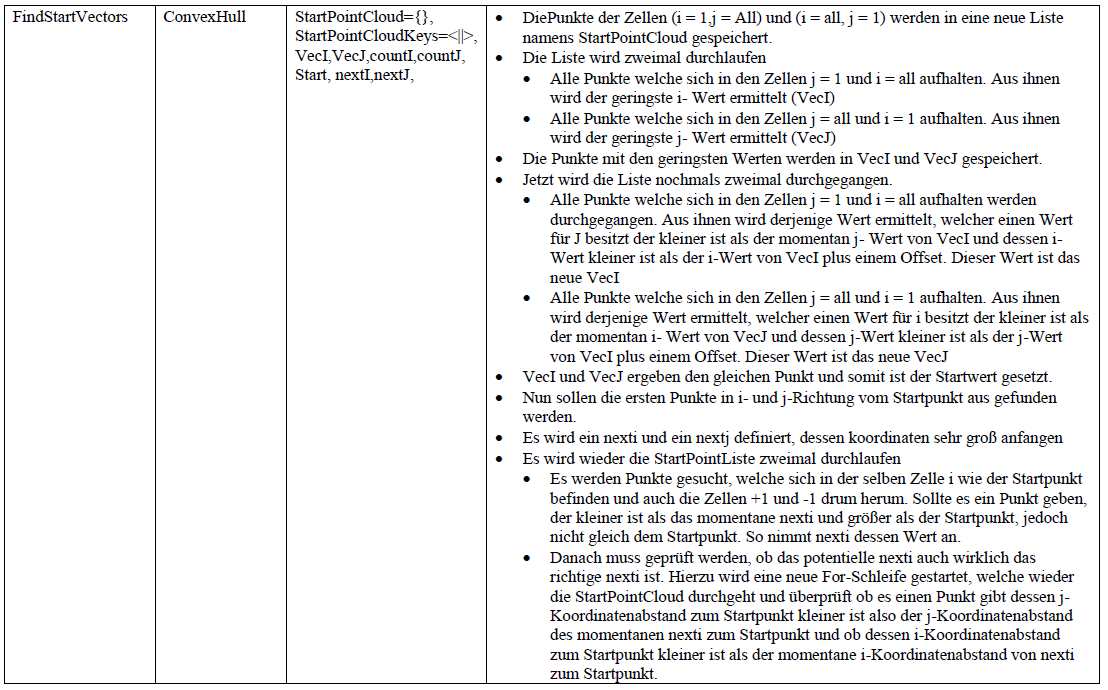
\includegraphics[width=1\linewidth]{images/KD2.png}
	\captionof{figure}{Klassendiagramm}
\end{minipage}
\begin{minipage}{\linewidth}
	\centering
	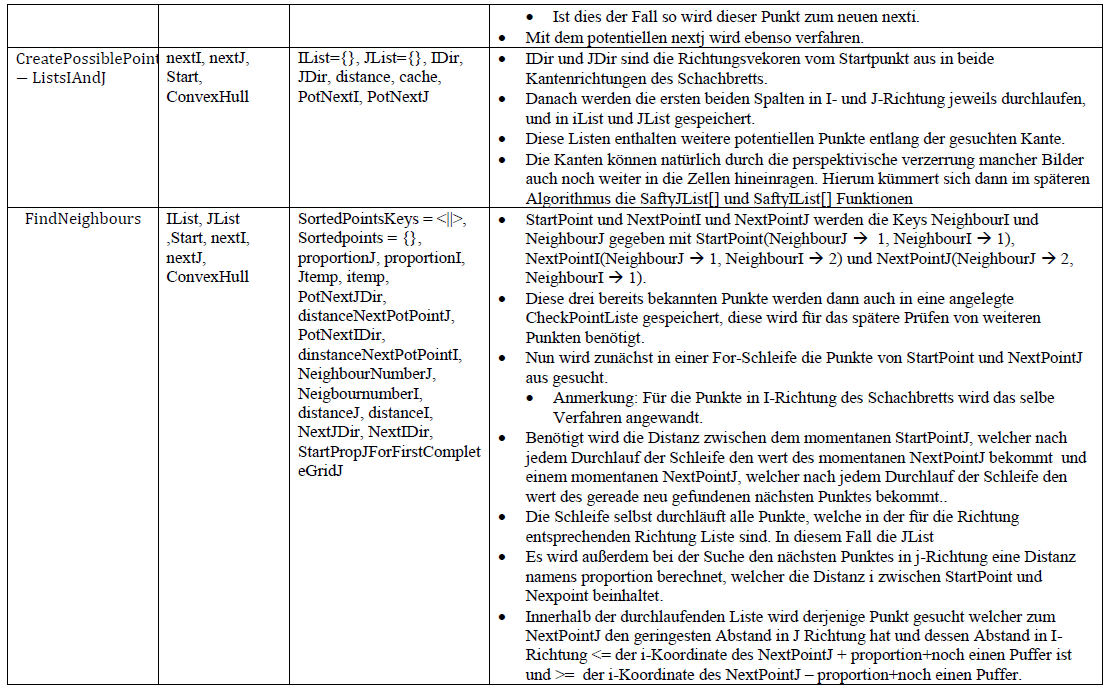
\includegraphics[width=1\linewidth]{images/KD3.png}
	\captionof{figure}{Klassendiagramm}
\end{minipage}
\begin{minipage}{\linewidth}
	\centering
	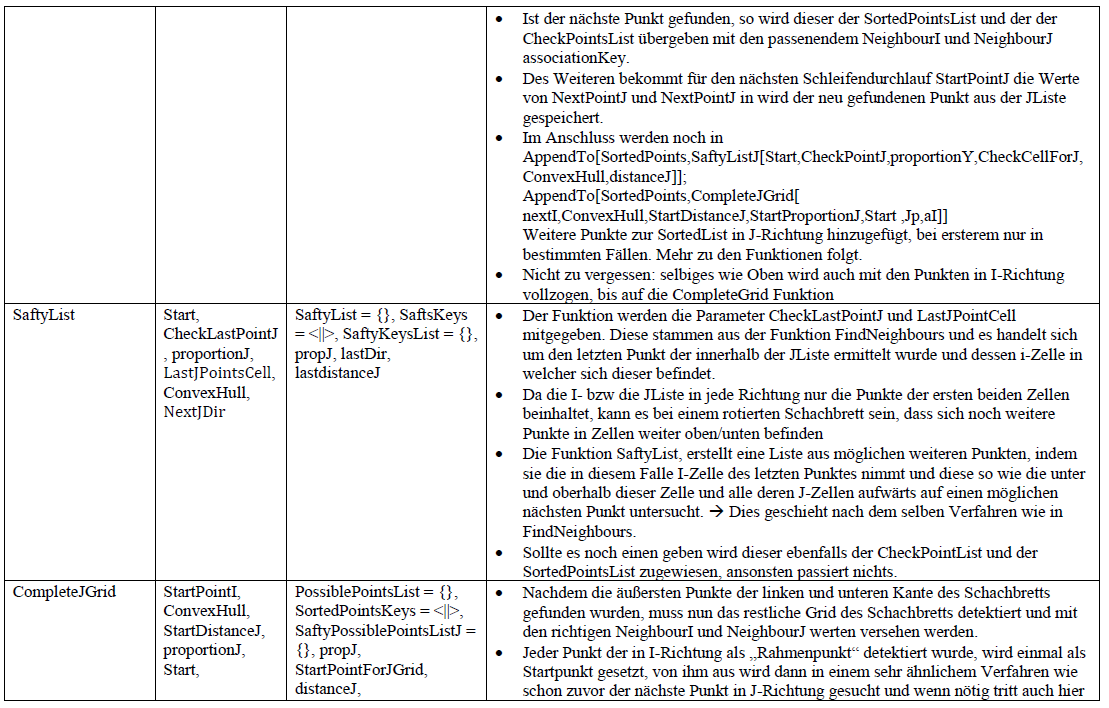
\includegraphics[width=1\linewidth]{images/KD4.png}
	\captionof{figure}{Klassendiagramm}
\end{minipage}
\begin{minipage}{\linewidth}
	\centering
	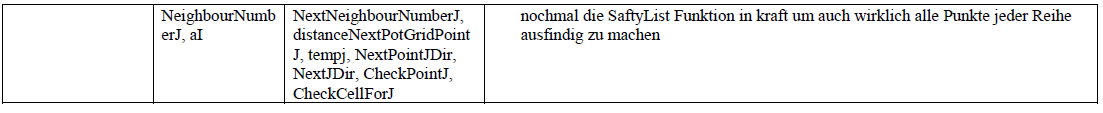
\includegraphics[width=1\linewidth]{images/KD5.png}
	\captionof{figure}{Klassendiagramm}
\end{minipage}\\


\begin{figure}[!htb]
	\minipage{0.48\textwidth}
	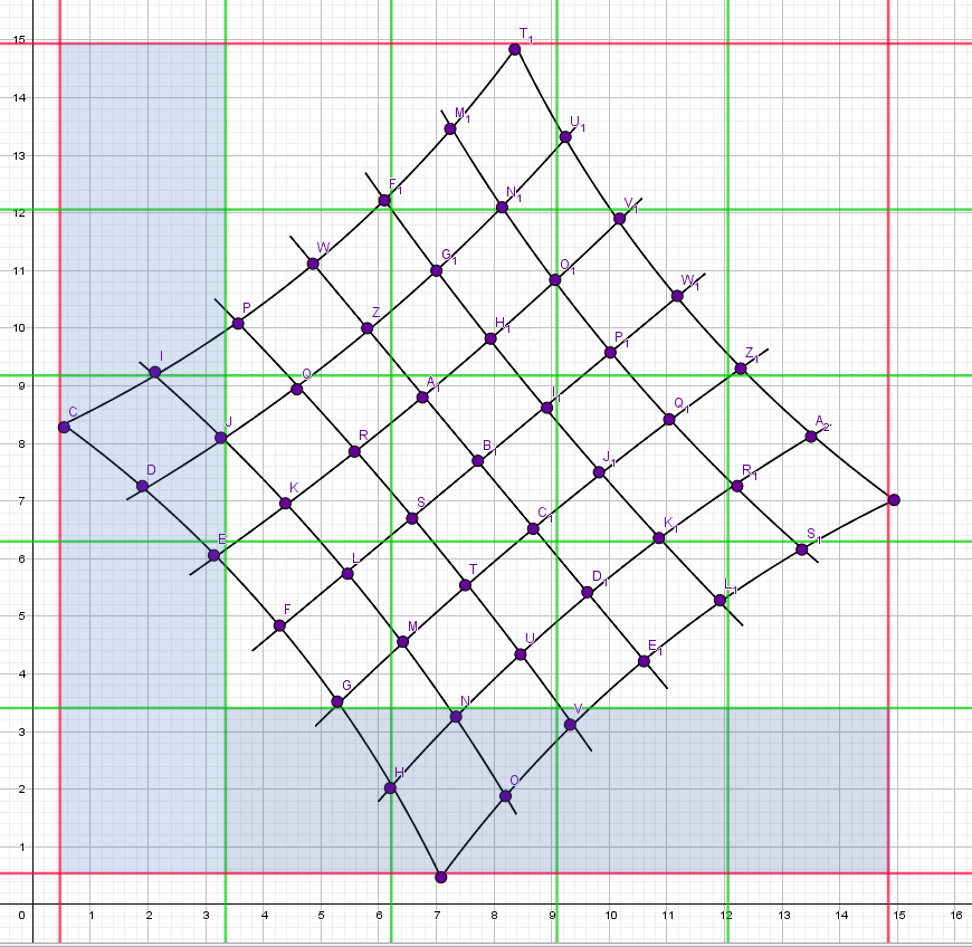
\includegraphics[width=\linewidth]{images/VerzeichnetesSchachbrett_0.png}
	\caption{}
	\label{fig:awesome_image1}
	\endminipage\hfill
	\minipage{0.48\textwidth}
	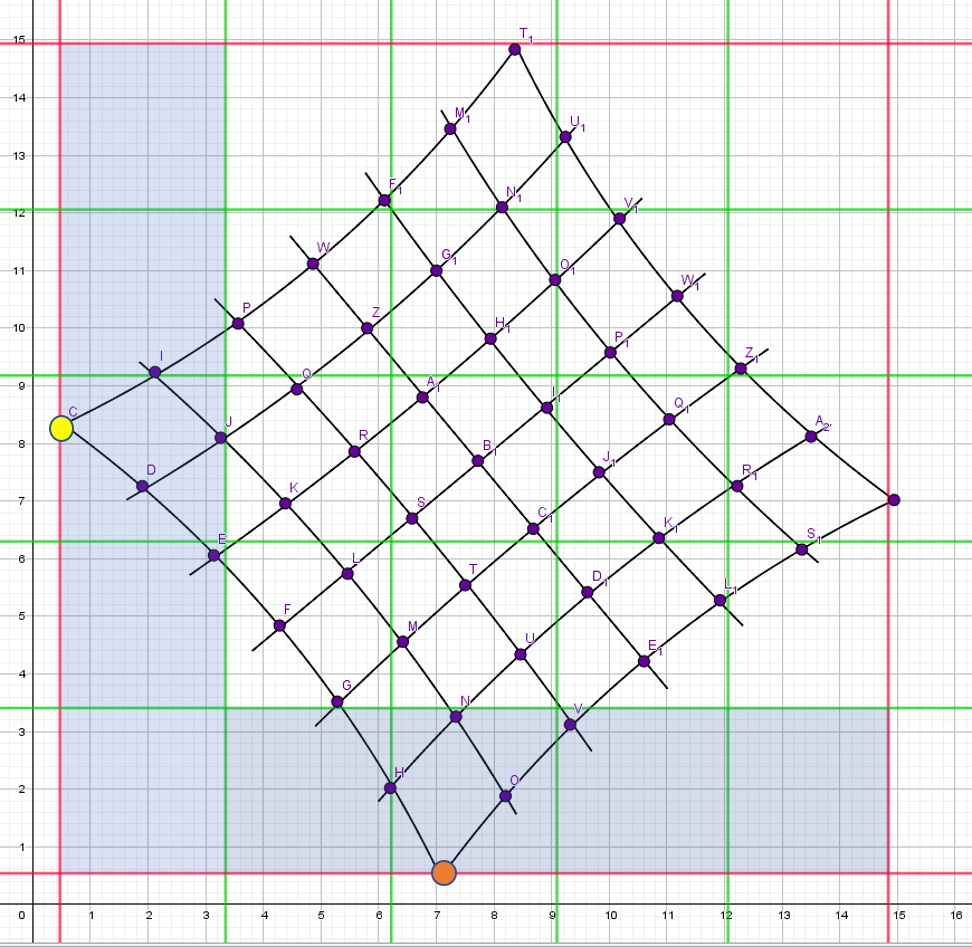
\includegraphics[width=\linewidth]{images/VerzeichnetesSchachbrett_1.png}
	\caption{}
	\label{fig:awesome_image2}
	\endminipage\hfill
	%	\caption{Die mit dem \textit{SURF}-Algorithmus gefundenen Punkte sind mit den gelben Ziffern im Bild gekennzeichnet}
\end{figure}

\begin{figure}[!htb]
	\minipage{0.48\textwidth}
	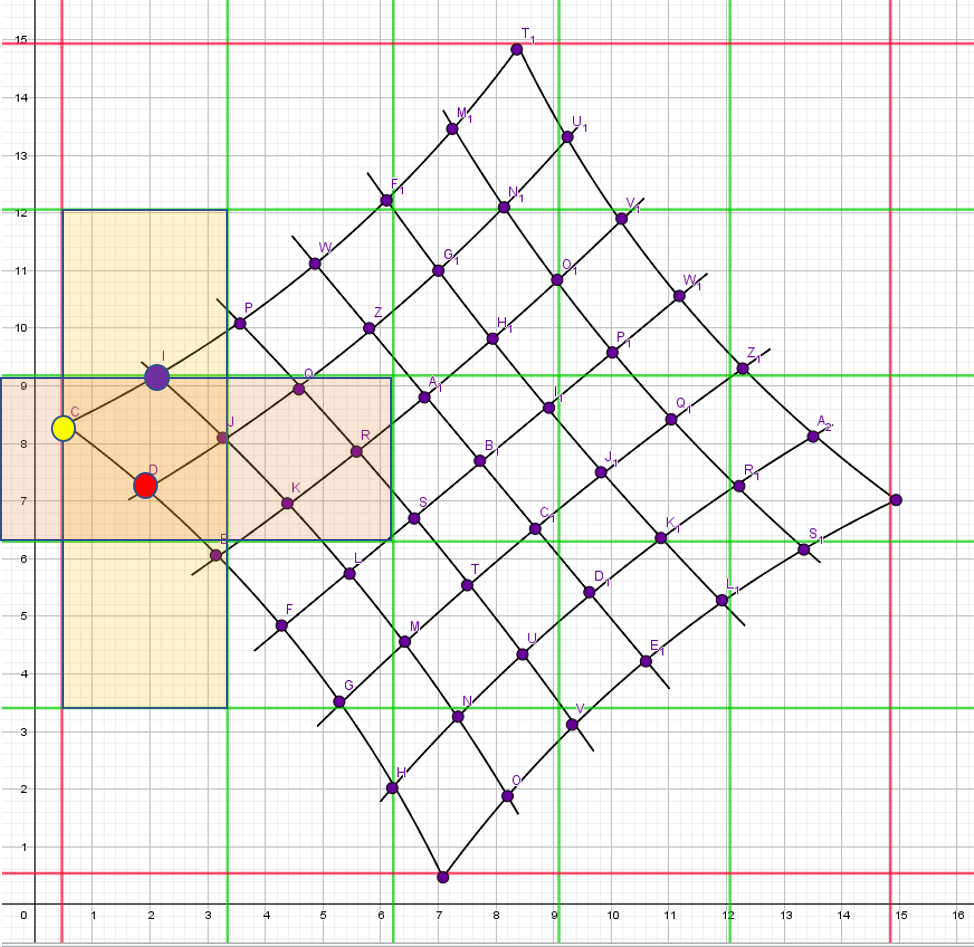
\includegraphics[width=\linewidth]{images/VerzeichnetesSchachbrett_2.png}
	\caption{}
	\label{fig:awesome_image1}
	\endminipage\hfill
	\minipage{0.48\textwidth}
	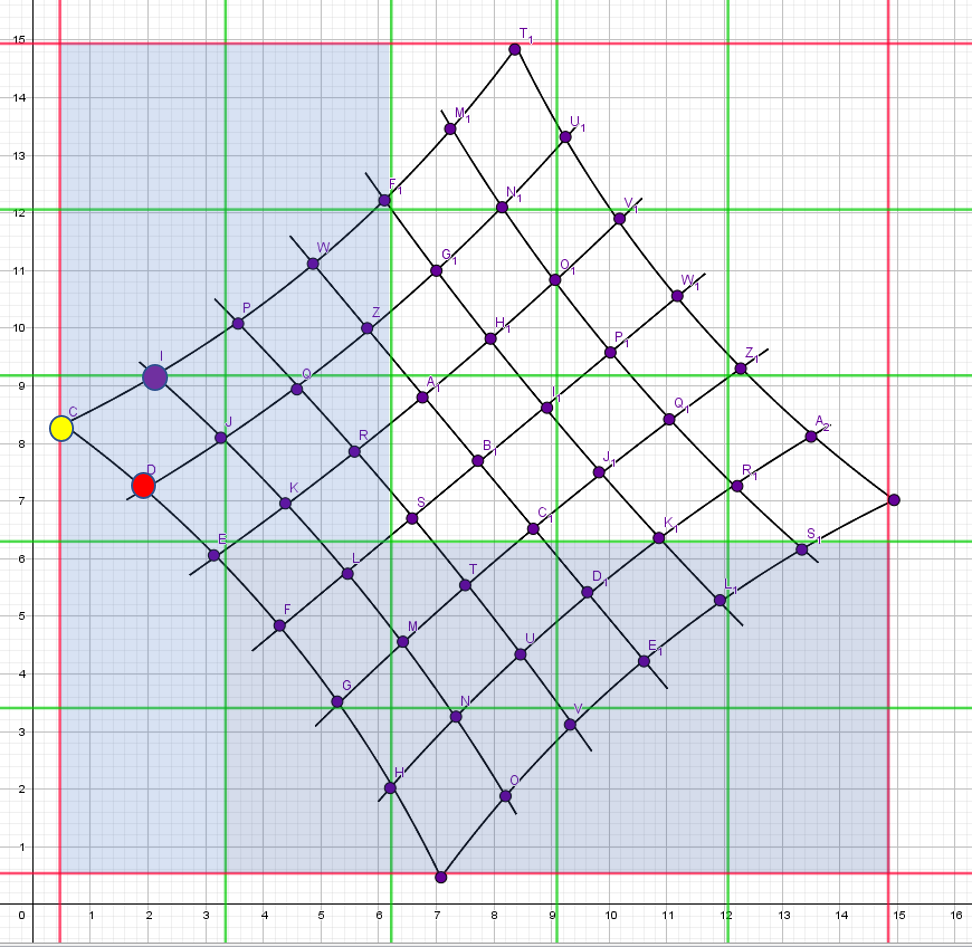
\includegraphics[width=\linewidth]{images/VerzeichnetesSchachbrett_3.png}
	\caption{}
	\label{fig:awesome_image2}
	\endminipage\hfill
	%	\caption{Die mit dem \textit{SURF}-Algorithmus gefundenen Punkte sind mit den gelben Ziffern im Bild gekennzeichnet}
\end{figure}

\begin{minipage}{\linewidth}
	\centering
	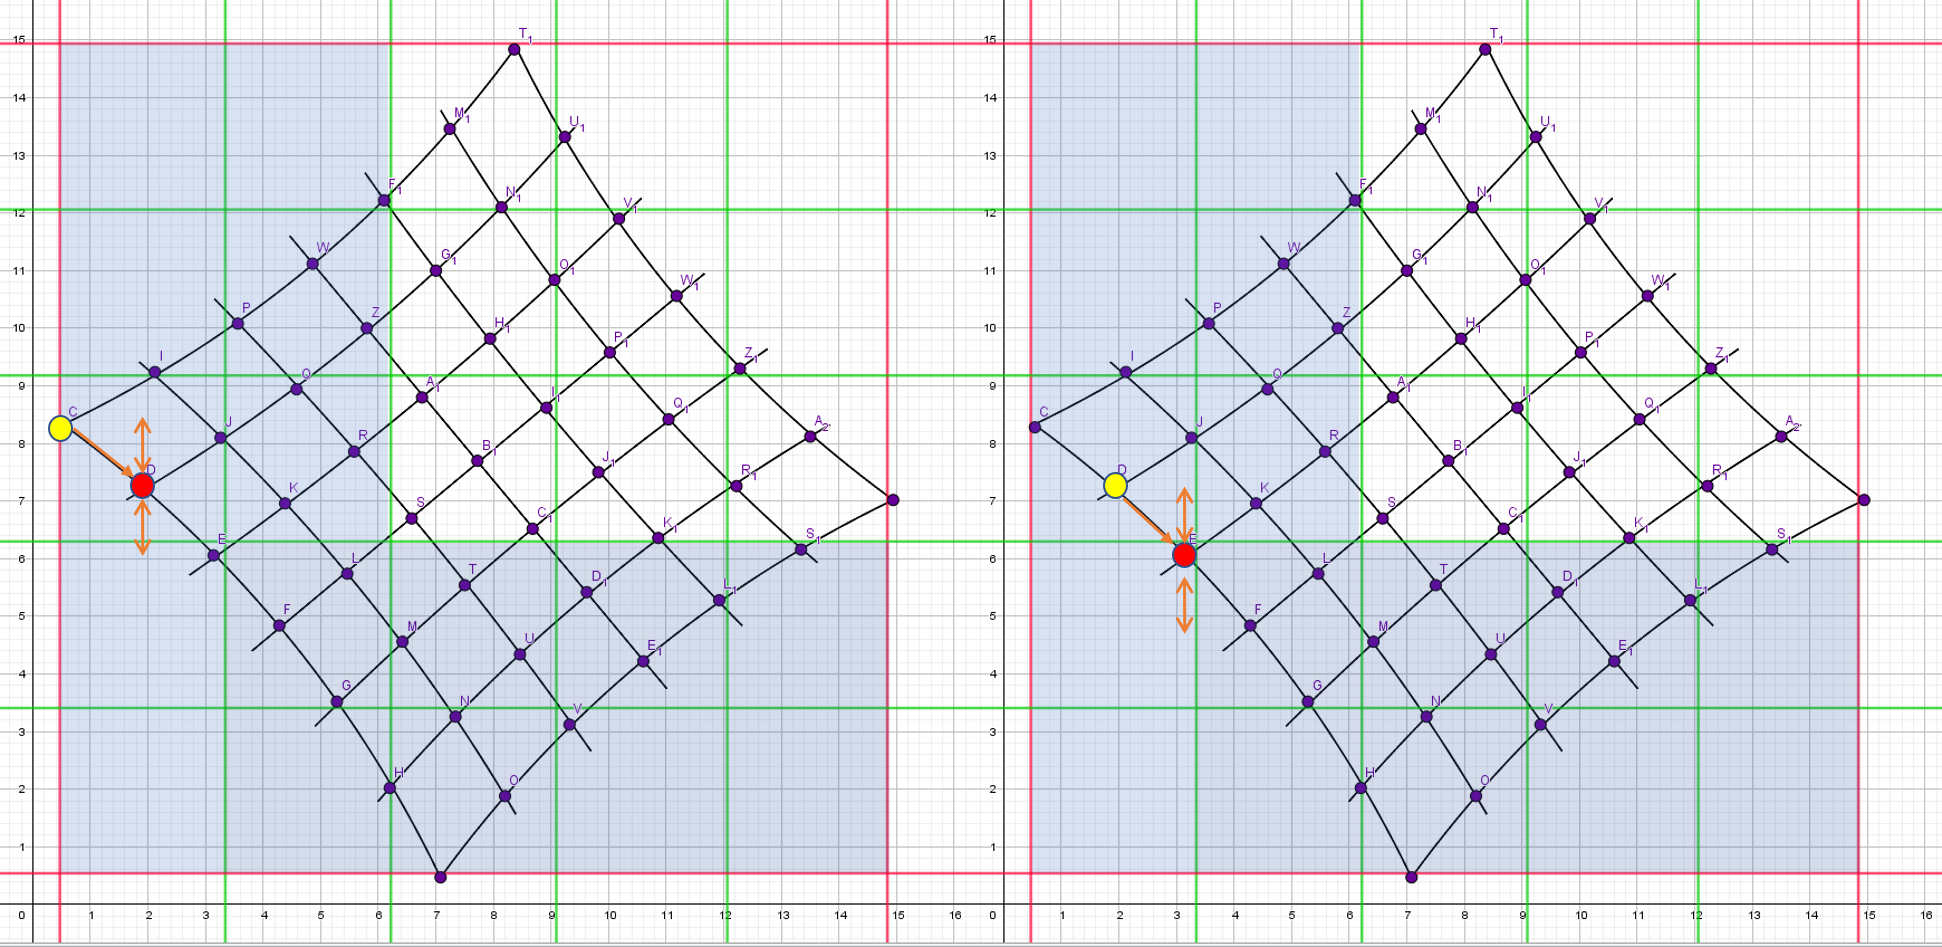
\includegraphics[width=1\linewidth]{images/VerzeichnetesSchachbrett_4.png}
	\captionof{figure}{Klassendiagramm}
\end{minipage}\\

\begin{minipage}{\linewidth}
	\centering
	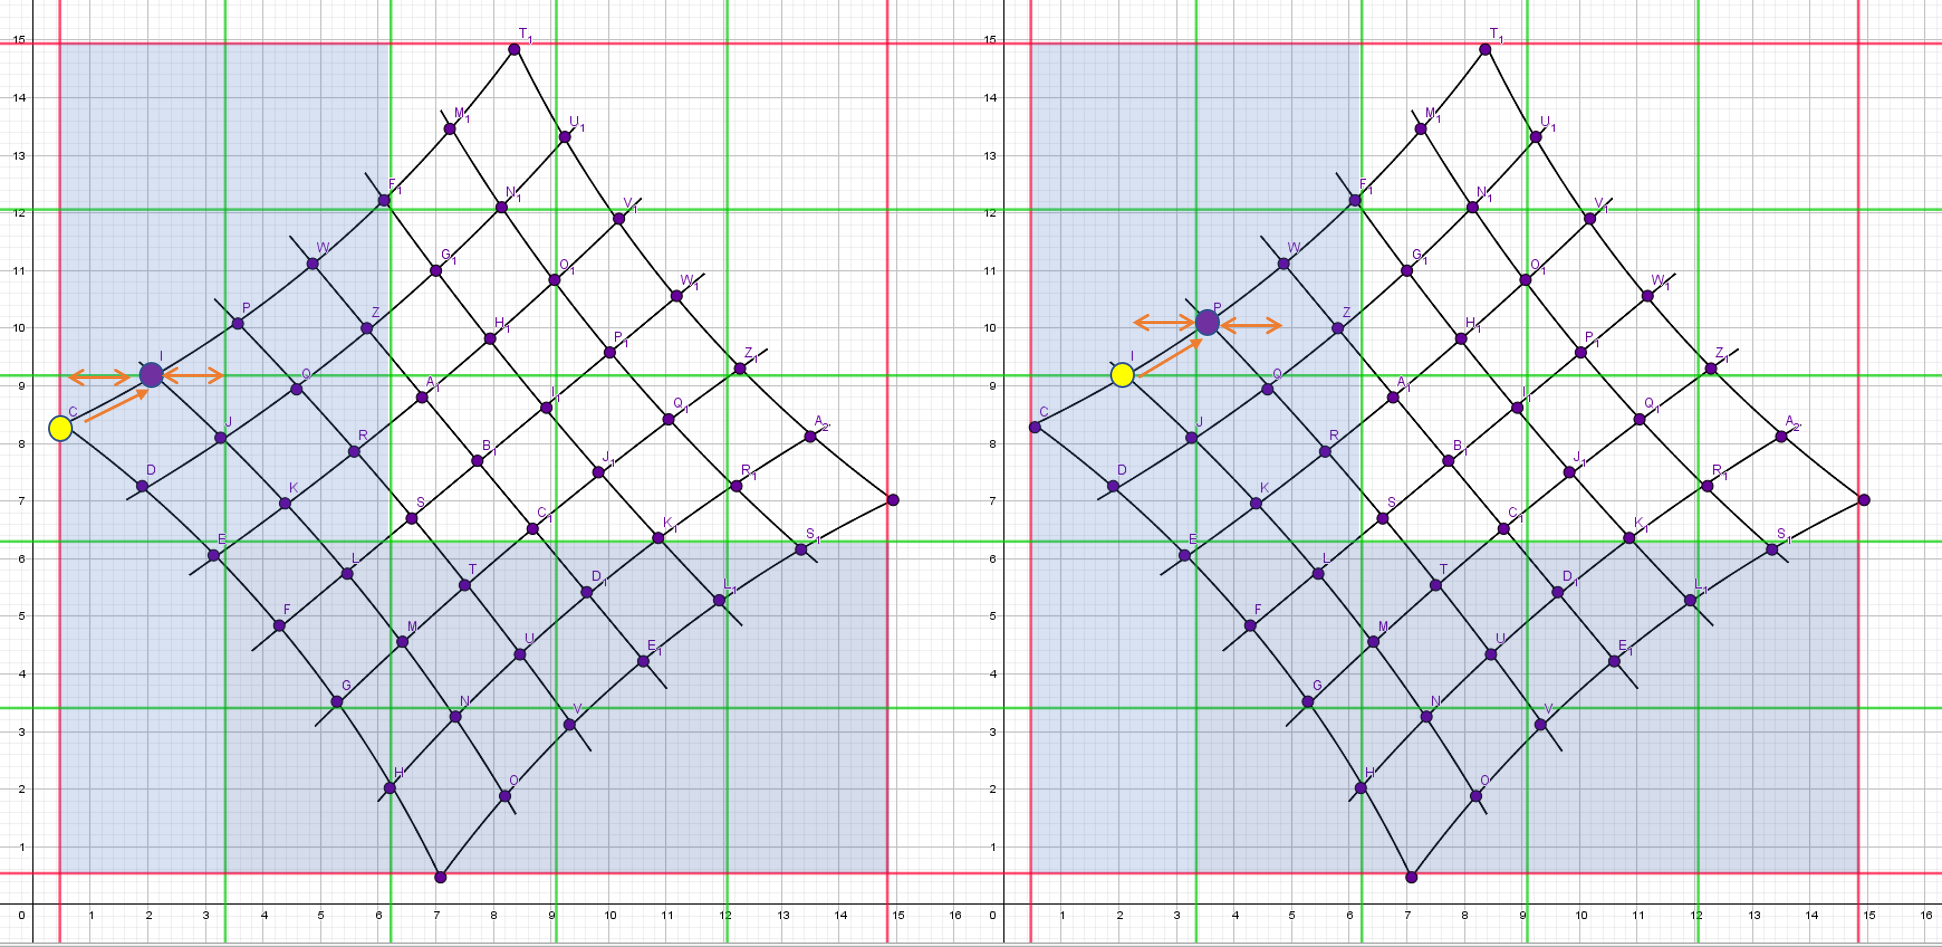
\includegraphics[width=1\linewidth]{images/VerzeichnetesSchachbrett_5.png}
	\captionof{figure}{Klassendiagramm}
\end{minipage}\\

\begin{minipage}{\linewidth}
	\centering
	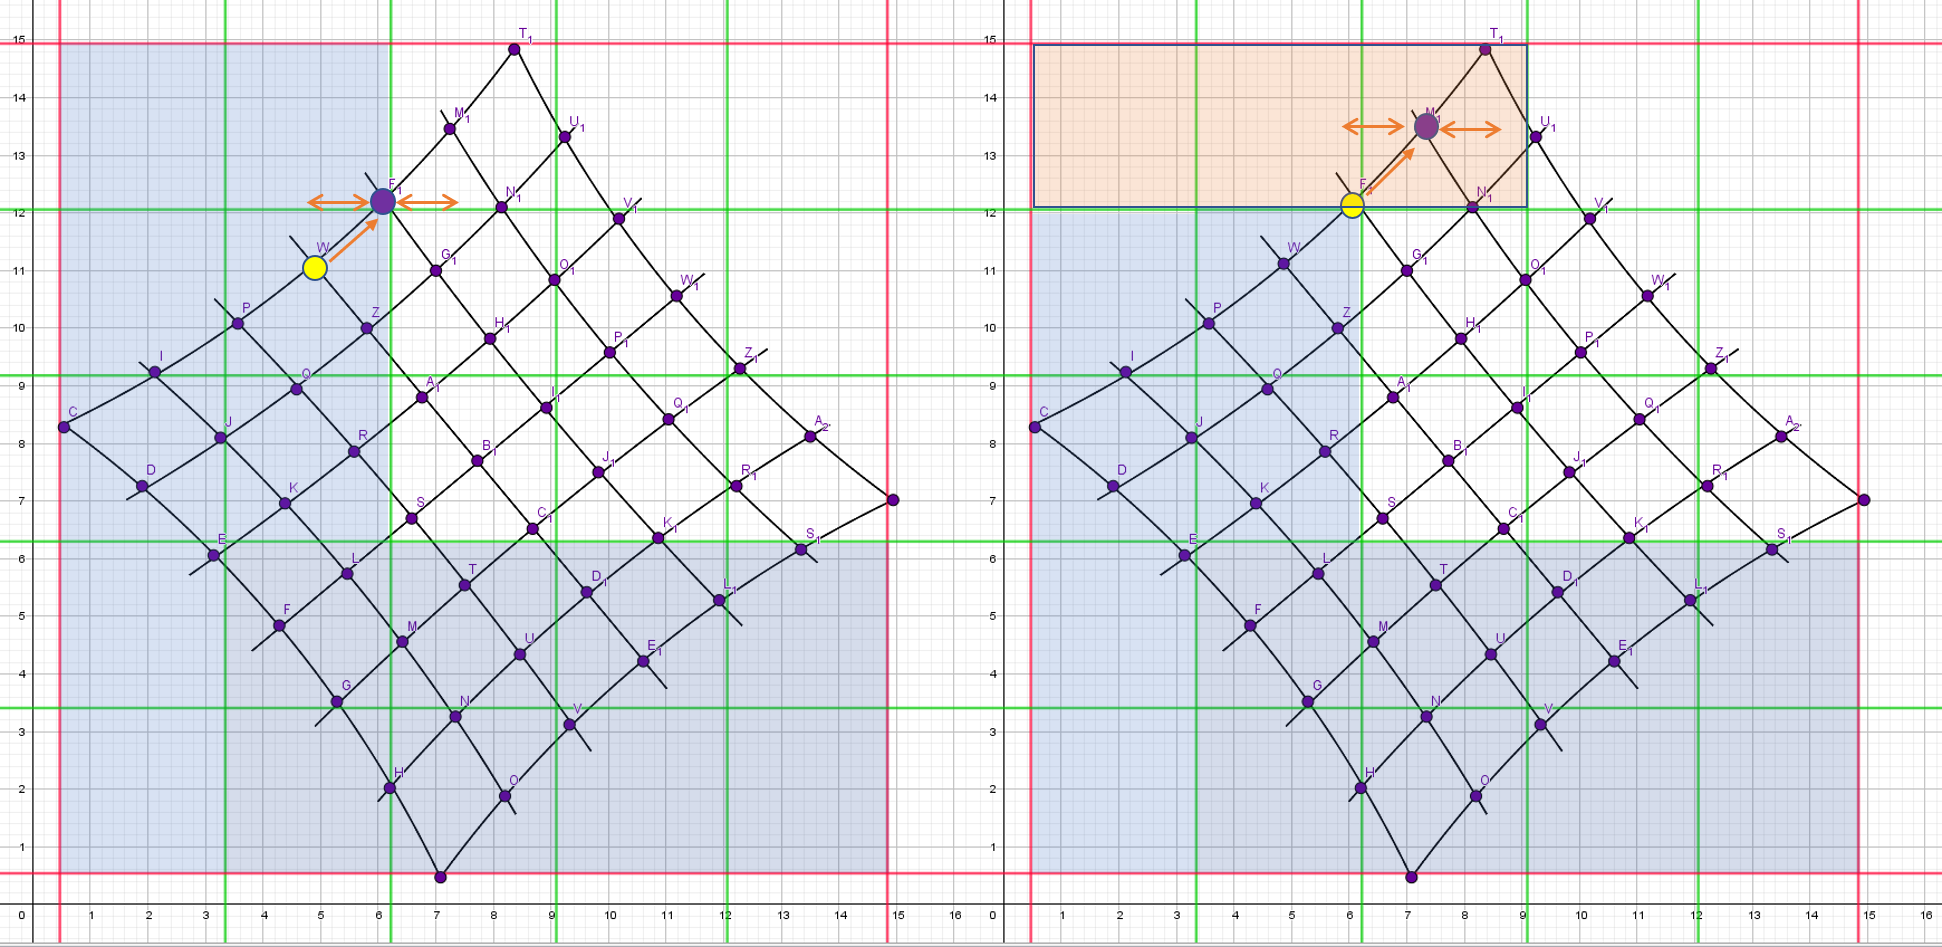
\includegraphics[width=1\linewidth]{images/VerzeichnetesSchachbrett_6.png}
	\captionof{figure}{Klassendiagramm}
\end{minipage}\\


\subsection{Beispiele}

In den folgenden Beispielen sieht man jeweils das Originalbild und ein Bild welches die durch den Algorithmus sortierten Punkte farbig ausgibt. Die grünen eingefärbten Punkte sind in den Bildern des Algorithmus die Nachbarn, welche sich in i-Richtung an der dritten Stelle befinden. Natürlich können auch andere Reihen oder auch einzelne Punkte abgefragt werden. 

\begin{figure}[!htb]
	\minipage{0.48\textwidth}
	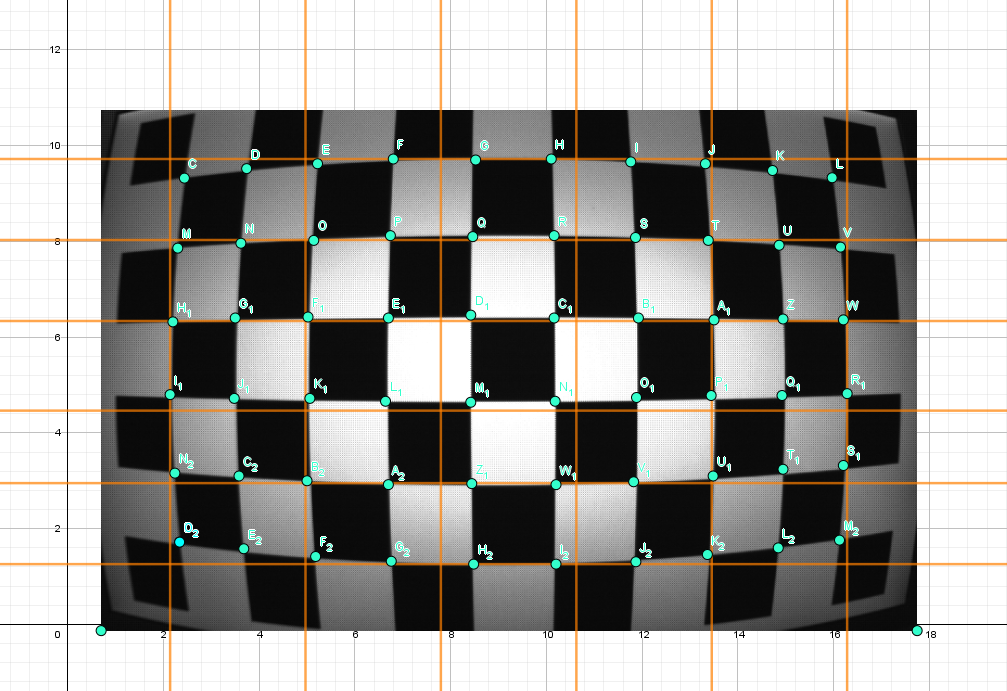
\includegraphics[width=\linewidth]{images/Tonnenverzeichnung.png}
	\caption{Bild eines Tonnenförmig verzeichneten Schachbretts}
	\label{fig:awesome_image1}
	\endminipage\hfill
	\minipage{0.48\textwidth}
	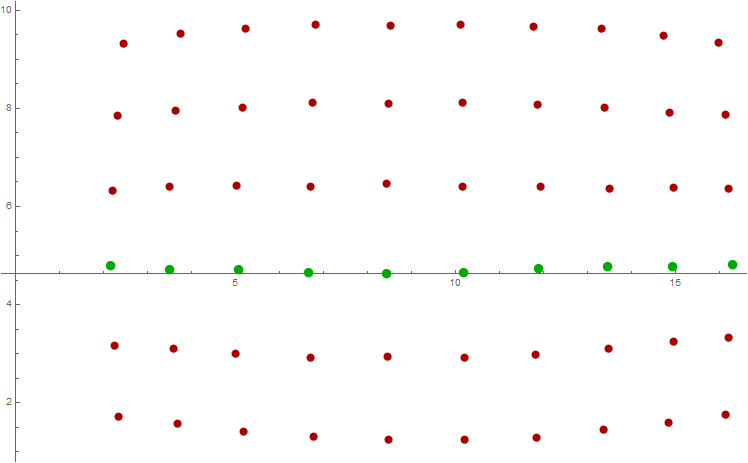
\includegraphics[width=\linewidth]{images/AlgTonnenverzeichnung.png}
	\caption{Algorithmisch detektierte Linie der dritten i-Reihe}
	\label{fig:awesome_image2}
	\endminipage\hfill
\end{figure}

%\begin{minipage}{\linewidth}
%	\centering
%	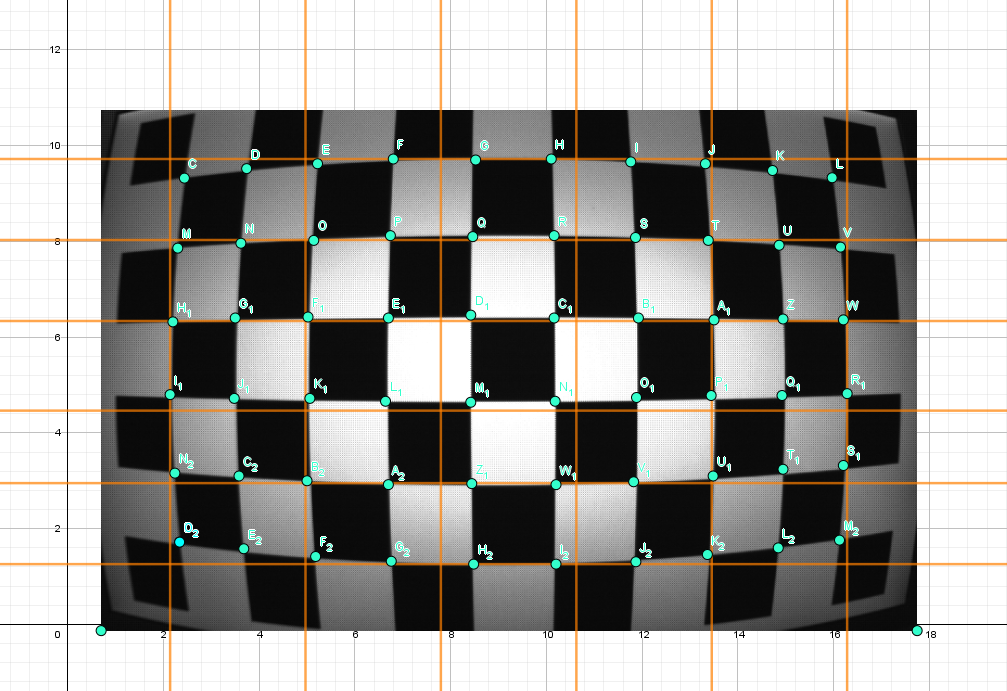
\includegraphics[width=1\linewidth]{images/Tonnenverzeichnung.png}
%	\captionof{figure}{Bild eines Tonnenförmig verzeichneten Schachbretts}
%\end{minipage}\\
%
%\begin{minipage}{\linewidth}
%	\centering
%	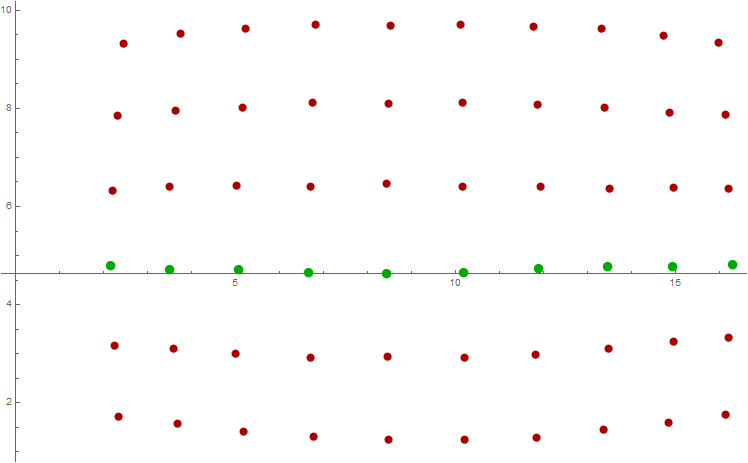
\includegraphics[width=1\linewidth]{images/AlgTonnenverzeichnung.png}
%	\captionof{figure}{Algorithmisch detektierte Linie der dritten i-Reihe}
%\end{minipage}\\\\

\begin{figure}[!htb]
	\minipage{0.48\textwidth}
	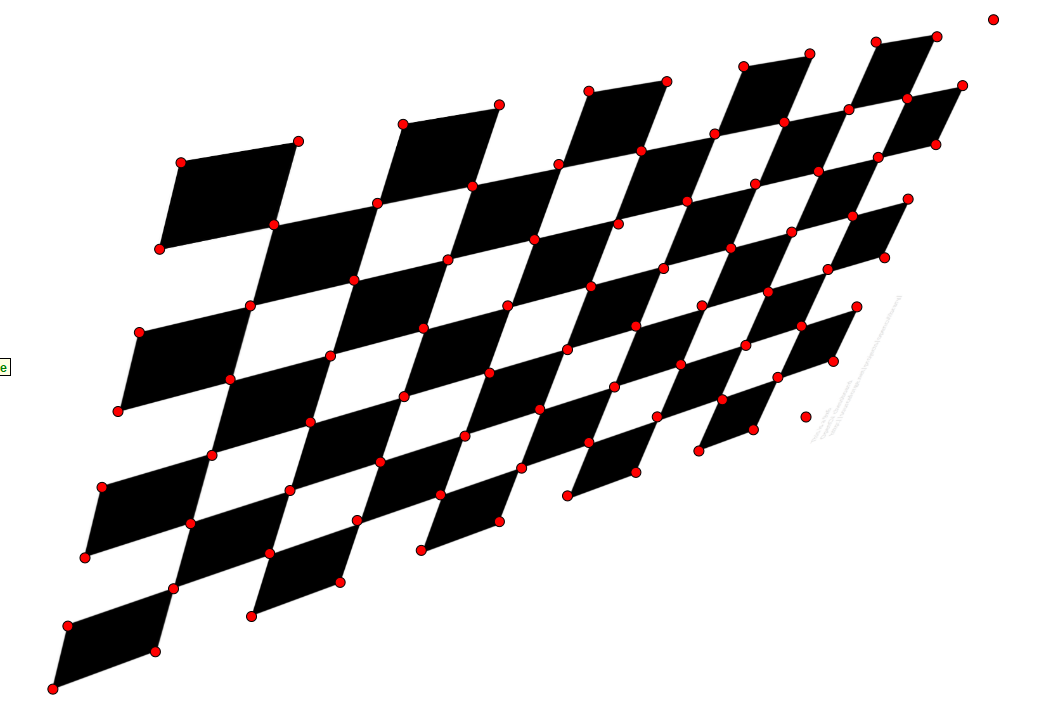
\includegraphics[width=\linewidth]{images/perspektivisch.png}
	\caption{Bild eines perspektivisch verzerrtem Schachbretts}
	\label{fig:awesome_image1}
	\endminipage\hfill
	\minipage{0.48\textwidth}
	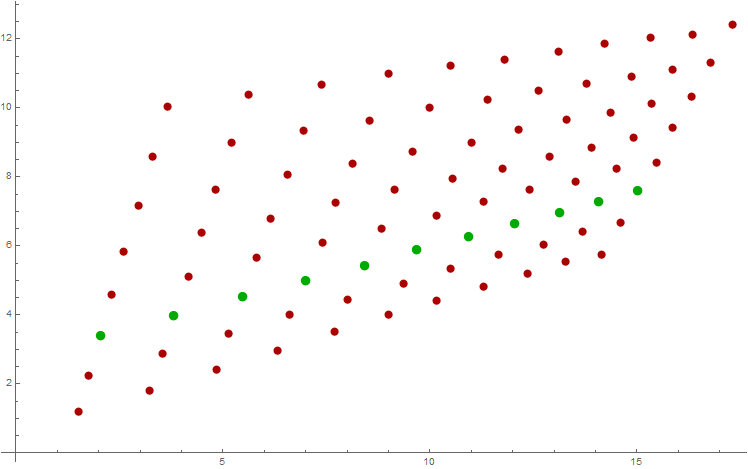
\includegraphics[width=\linewidth]{images/AlgPerspektifisch.png}
	\caption{Algorithmisch detektierte Linie der dritten i-Reihe}
	\label{fig:awesome_image2}
	\endminipage\hfill
\end{figure}

%\begin{minipage}{\linewidth}
%	\centering
%	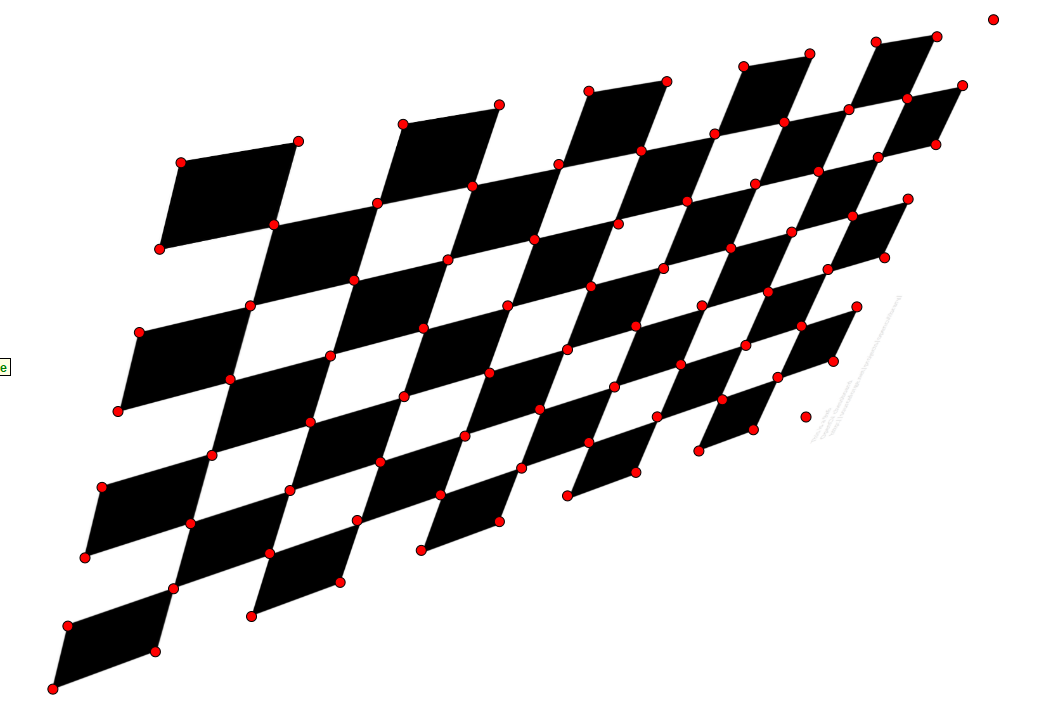
\includegraphics[width=1\linewidth]{images/perspektivisch.png}
%	\captionof{figure}{Bild eines perspektivisch verzerrtem Schachbretts}
%\end{minipage}\\
%
%\begin{minipage}{\linewidth}
%	\centering
%	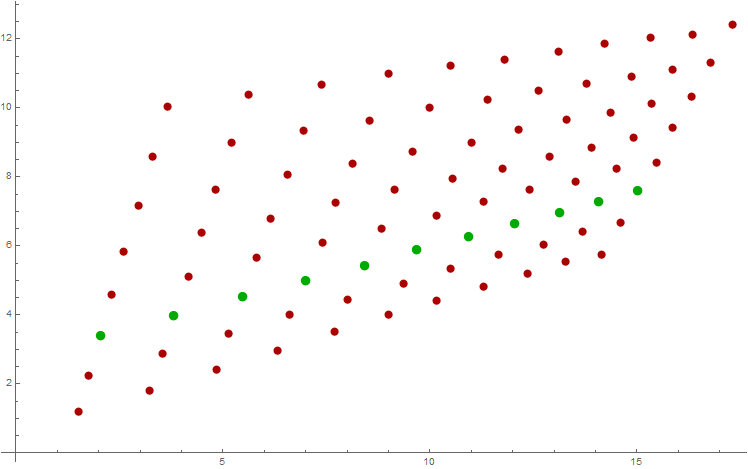
\includegraphics[width=1\linewidth]{images/AlgPerspektifisch.png}
%	\captionof{figure}{Algorithmisch detektierte Linie der dritten i-Reihe}
%\end{minipage}\\\\

\begin{figure}[!htb]
	\minipage{0.48\textwidth}
	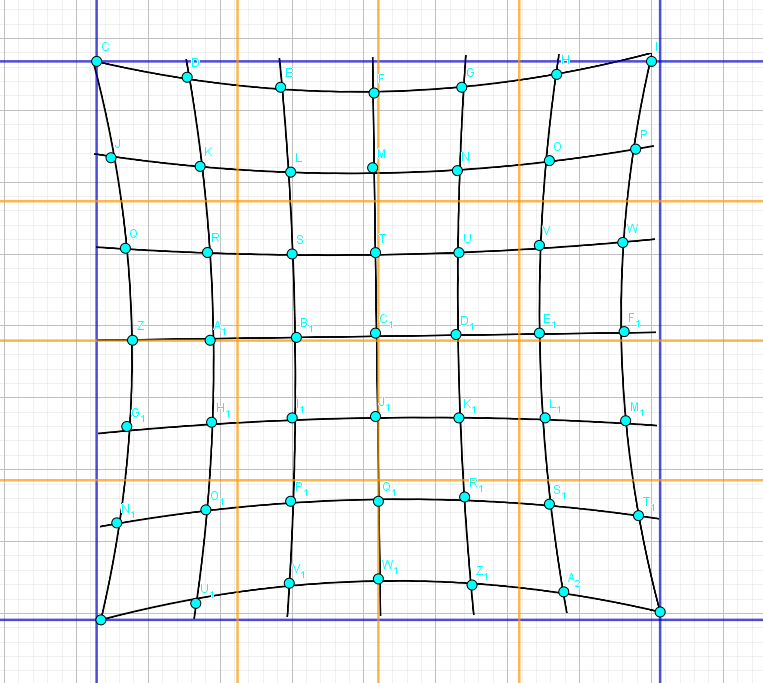
\includegraphics[width=\linewidth]{images/KissenVerzeichnung.png}
	\caption{Bild eines Kissenförmig verzeichnetem Schachbretts}
	\label{fig:awesome_image1}
	\endminipage\hfill
	\minipage{0.48\textwidth}
	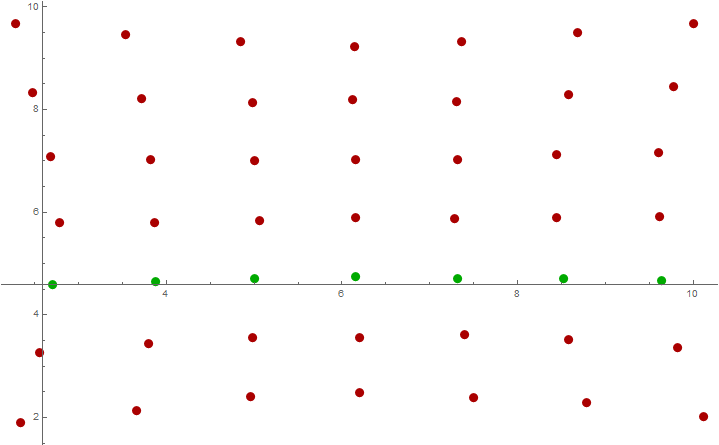
\includegraphics[width=\linewidth]{images/AlgKissen.png}
	\caption{Algorithmisch detektierte Linie der dritten i-Reihe}
	\label{fig:awesome_image2}
	\endminipage\hfill
\end{figure}

%\begin{minipage}{\linewidth}
%	\centering
%	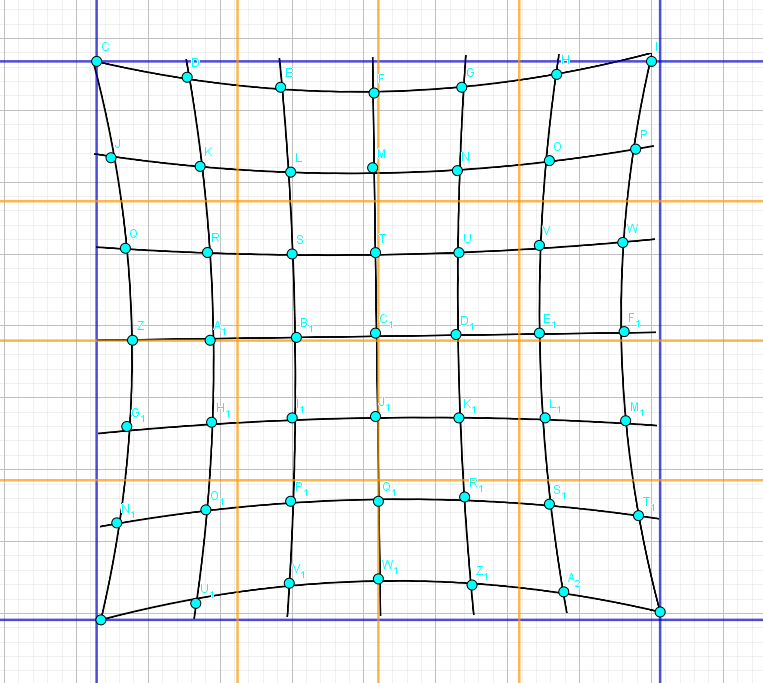
\includegraphics[width=.8\linewidth]{images/KissenVerzeichnung.png}
%	\captionof{figure}{Bild eines Kissenförmig verzeichnetem Schachbretts}
%\end{minipage}\\
%
%\begin{minipage}{\linewidth}
%	\centering
%	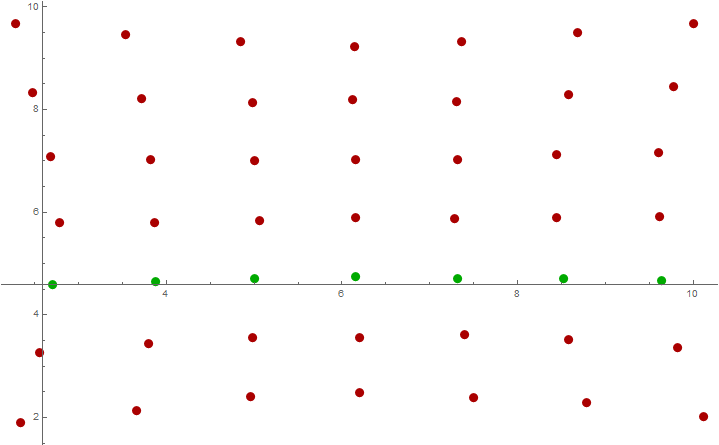
\includegraphics[width=1\linewidth]{images/AlgKissen.png}
%	\captionof{figure}{Algorithmisch detektierte Linie der dritten i-Reihe}
%\end{minipage}\\\\

%\begin{minipage}{\linewidth}
%	\centering
%	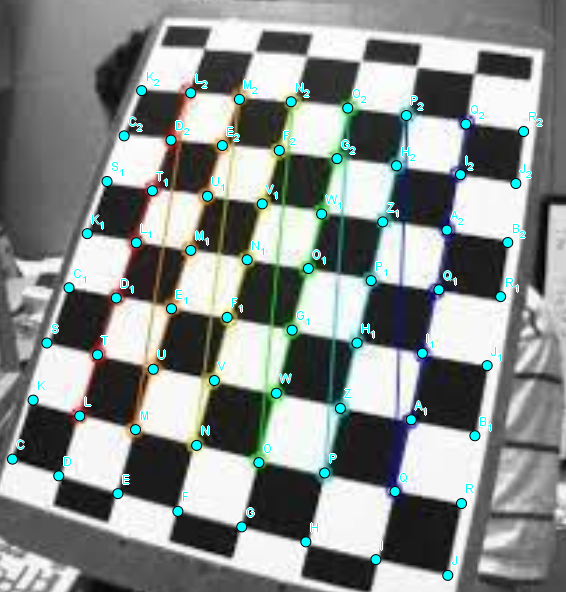
\includegraphics[width=.8\linewidth]{images/TonnePers.png}
%	\captionof{figure}{Bild eines Tonnenförmig verzeichnetem leicht perspektivisch verzerrtem Schachbretts}
%\end{minipage}\\
%
%\begin{minipage}{\linewidth}
%	\centering
%	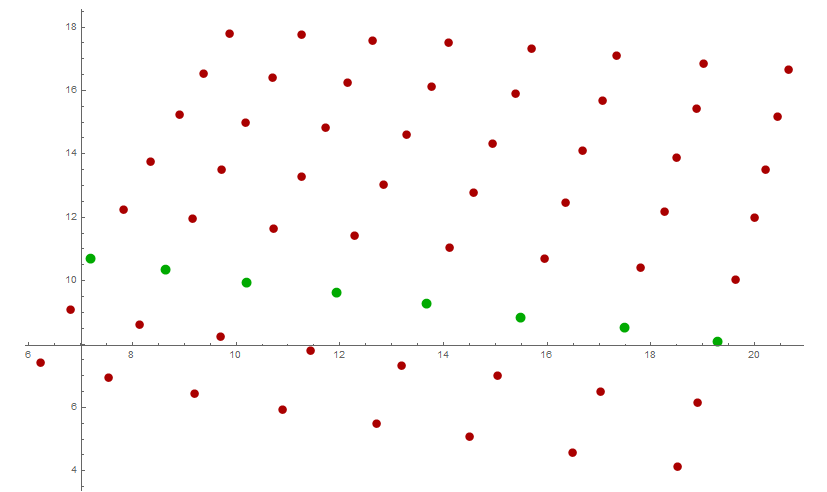
\includegraphics[width=1\linewidth]{images/AlgTonnePers.png}
%	\captionof{figure}{Algorithmisch detektierte Linie der dritten i-Reihe}
%\end{minipage}\\\\

\begin{figure}[!htb]
	\minipage{0.48\textwidth}
	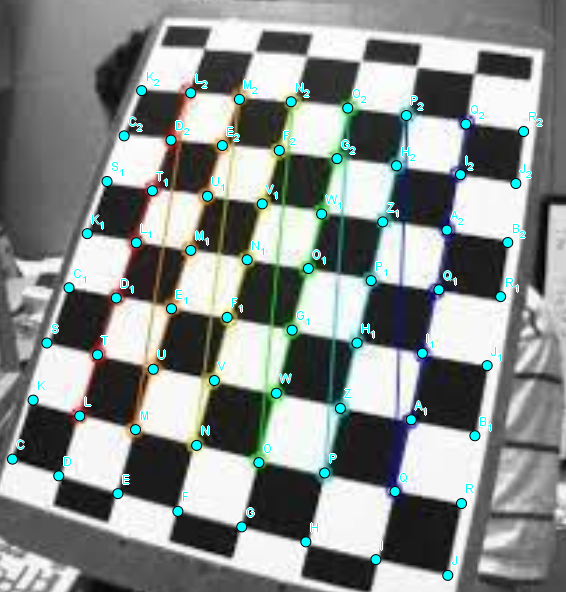
\includegraphics[width=\linewidth]{images/TonnePers.png}
	\caption{Bild eines Tonnenförmig verzeichnetem leicht perspektivisch verzerrtem Schachbretts(GRFIK AUSTAUSCHEN BILD IS KACKE)}
	\label{fig:awesome_image1}
	\endminipage\hfill
	\minipage{0.48\textwidth}
	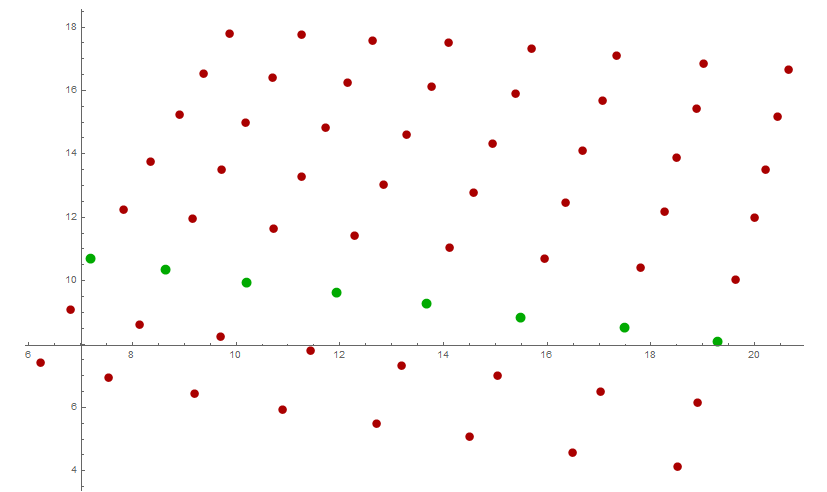
\includegraphics[width=\linewidth]{images/AlgTonnePers.png}
	\caption{Algorithmisch detektierte Linie der dritten i-Reihe}
	\label{fig:awesome_image2}
	\endminipage\hfill
\end{figure}

%
%\begin{minipage}{\linewidth}
%	\centering
%	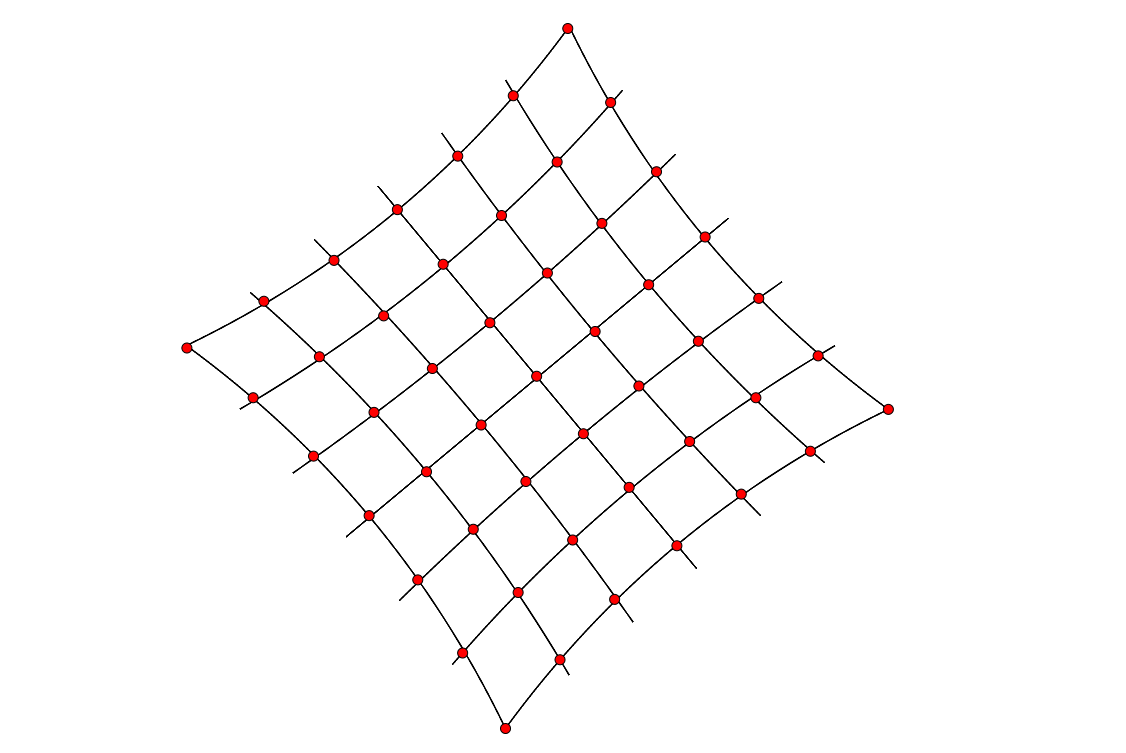
\includegraphics[width=.8\linewidth]{images/extrBsp.png}
%	\captionof{figure}{Kissenverzeichnung start rotiert}
%\end{minipage}\\
%
%\begin{minipage}{\linewidth}
%	\centering
%	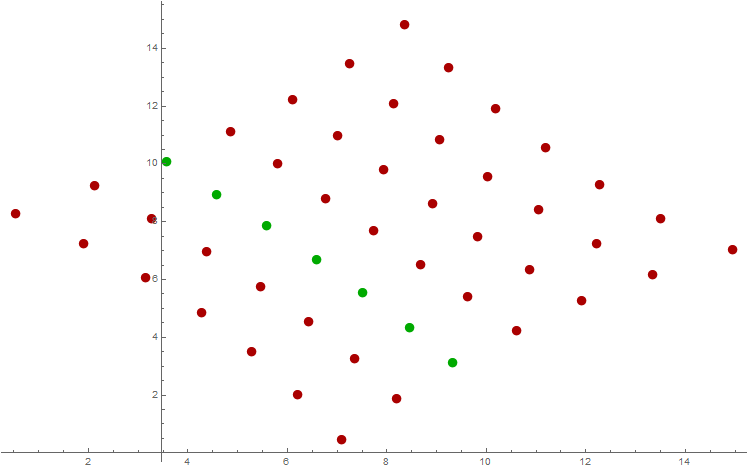
\includegraphics[width=1\linewidth]{images/AlgExtrBsp.png}
%	\captionof{figure}{Kissenverzeichnung start rotiert bisher gefundene Punkte}
%\end{minipage}\\\\

\begin{figure}[!htb]
	\minipage{0.48\textwidth}
	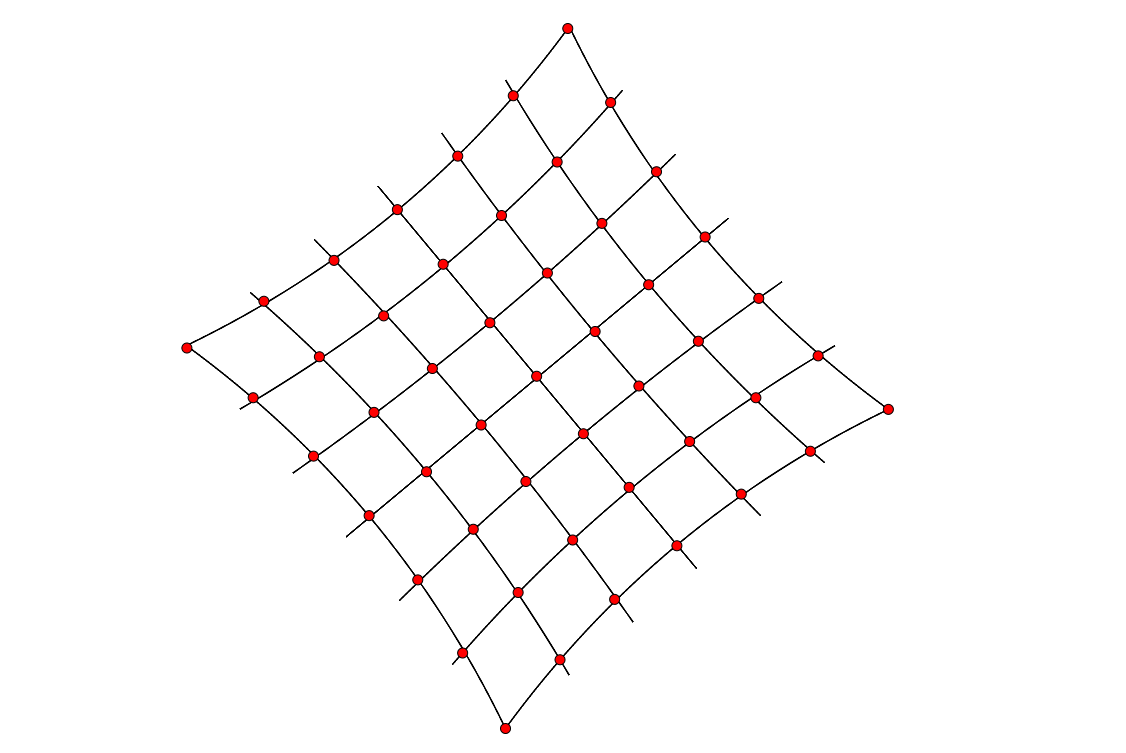
\includegraphics[width=\linewidth]{images/extrBsp.png}
	\caption{Bild eines Tonnenförmig verzeichnetem leicht perspektivisch verzerrtem Schachbretts}
	\label{fig:awesome_image1}
	\endminipage\hfill
	\minipage{0.48\textwidth}
	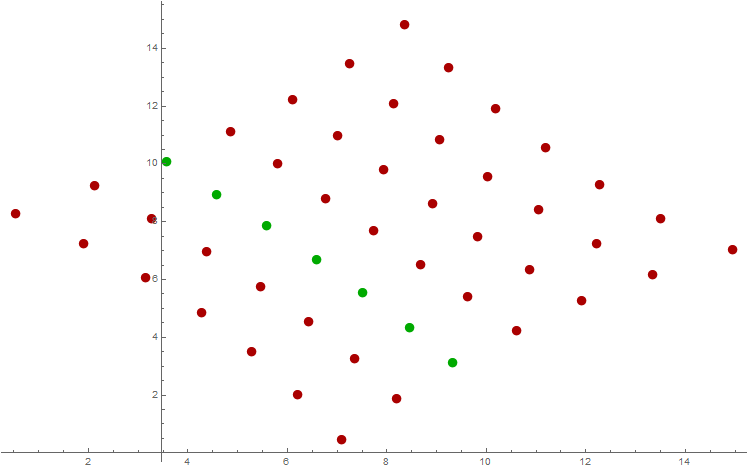
\includegraphics[width=\linewidth]{images/AlgExtrBsp.png}
	\caption{Algorithmisch detektierte Linie der dritten i-Reihe}
	\label{fig:awesome_image2}
	\endminipage\hfill
\end{figure}

%\pagebreak
%\subsection{Weiteres Vorgehen/ Was fehlt noch}
%
%Was nun noch in den Algorithmus eingebaut werden muss ist eine \textit{Saftylist}-Funktion welche auch in i-Richtung wirkt. Des Weitern muss davon ausgeganegn werden, dass der voranlaufgende Algorithmus zu Auffindung der Punkte, nicht immer alle Punkte detektiert. Es muss also noch eine Funktion geschrieben werden, welche zunächst prüft, ob es noch einen nächsten Punkt gibt, wenn dies nicht der Fall ist wird ein vorläufiger Punkt an die Stelle gesetzt, an welcher der Punkt sich befinden sollte und von diesem aus weiter geprüft ob es noch einen gibt. Sollte dies der Fall sein, so wird ab dem nächsten real gefundenen Punkt weiter gesucht und der selbst erzeugte Punkt wird als ''fake'' Punkt eingesetzt. Sollte nach dem erstellten Punkt weiterhin keiner folgen, kann man überlegen den test nochmals vom selbst erstellten Punkt aus auszuführen, oder es dabei zu belassen. \\
%
%(VERBESSERN)
%Des Weiteren muss nochmal genau ermittelt werden warum es bei einem sehr extremen Fall wie in der folgenden Abbildung noch nicht ganz funktioniert. Die Vermutung ist, dass hier noch mit SaftyFunktionen in i-Richtungen hantiert werden muss. 
%
%
%
%Als letztes werden die Pufferwerte momentan noch hart gecoded, diese sollen in Zukunft aus den Zahlenbereichen in welchen sich die Punkte aufhalten ausgerechnet werden.
